\chapter{Our Datasets}
In this appendix we show the complete datasets that we used in our study. Table \ref{complete_astrodata} shows the full dataset of \cite{osman}. The NaN value indicates a missing value.
% Please add the following required packages to your document preamble:
% \usepackage{booktabs}
\begin{table}[]
	\centering
	\caption{Complete astrogeodetic data of \cite{osman}}
	\label{complete_astrodata}
	\begin{tabular}{@{}lll@{}}
		\toprule
		latitutde & longitude & geoid height \\ \midrule
		22.169    & 31.489    & 10.000       \\
		20.136    & 30.662    & 9.556        \\
		18.473    & 30.840    & 10.198       \\
		17.051    & 31.272    & 10.199       \\
		14.496    & 30.251    & 14.180       \\
		13.832    & 29.654    & 15.833       \\
		13.233    & 30.110    & 15.354       \\
		12.866    & 29.956    & 15.647       \\
		12.776    & 30.853    & 14.453       \\
		11.604    & 30.411    & 15.387       \\
		10.823    & 31.113    & 14.851       \\
		10.279    & 30.980    & 15.346       \\
		10.247    & 31.067    & 15.188       \\
		8.619     & 31.402    & 15.332       \\
		7.071     & 31.319    & 13.970       \\
		5.805     & 31.783    & 11.396       \\
		4.701     & 31.779    & 14.180       \\
		14.840    & 34.088    & 12.449       \\
		15.511    & 36.253    & 12.683       \\
		16.615    & 36.254    & 12.745       \\
		17.593    & 36.038    & 11.665       \\
		18.710    & 37.102    & 6.847        \\
		19.501    & 37.260    & 6.133        \\
		20.337    & 37.107    & 7.051        \\
		21.087    & 37.107    & 6.440        \\
		22.314    & 36.513    & 9.930        \\
		22.541    & 35.894    & 12.432       \\
		15.526    & 32.582    & NaN          \\
		18.172    & 37.559    & 7.384        \\
		18.114    & 36.312    & 13.107       \\
		17.388    & 37.355    & 11.026       \\
		15.721    & 31.761    & 11.939       \\
		16.027    & 31.817    & 11.713       \\
		15.716    & 32.414    & 11.318       \\
		16.242    & 32.681    & 10.689       \\
		16.164    & 32.756    & 10.631       \\
		14.858    & 34.963    & 12.301       \\
		13.404    & 29.368    & 16.498       \\
		13.273    & 28.811    & 17.360       \\
		13.239    & 28.424    & 17.432       \\
		13.368    & 27.976    & 17.699       \\
		13.439    & 27.602    & 18.221       \\
		13.664    & 26.446    & 19.149       \\
		13.660    & 25.768    & 20.917       \\
		13.566    & 25.221    & 22.669       \\
		13.417    & 24.733    & 24.250       \\ \bottomrule
	\end{tabular}
\end{table}

% Please add the following required packages to your document preamble:
% \usepackage{booktabs}
\begin{table}[]
	\centering
	\caption{Full GPS/leveling dataset of Khartoum \citep{ahmed_msc}}
	\label{table:khartoum_gps_leveling_data}
	\begin{tabular}{@{}lll@{}}
		\toprule
		latitude & longitude & geoid height \\ \midrule
		16.172   & 32.153    & 3.573        \\
		15.822   & 32.313    & 2.998        \\
		15.890   & 32.684    & 3.619        \\
		16.077   & 32.722    & 3.119        \\
		15.811   & 33.087    & 2.175        \\
		15.809   & 32.900    & 2.285        \\
		15.613   & 32.808    & 2.020        \\
		16.352   & 31.965    & 4.174        \\
		15.848   & 32.517    & 3.078        \\
		16.119   & 32.531    & 2.263        \\
		15.992   & 32.340    & 3.210        \\
		15.810   & 32.154    & 3.210        \\
		16.113   & 31.965    & 3.197        \\
		15.993   & 32.901    & 3.254        \\
		15.988   & 32.144    & 3.447        \\
		15.470   & 33.080    & 2.297        \\
		15.651   & 32.388    & 2.810        \\
		15.721   & 32.514    & 2.655        \\
		16.139   & 32.638    & 2.420        \\
		15.607   & 32.518    & 2.673        \\
		15.599   & 32.108    & 2.538        \\
		15.524   & 32.577    & 2.599        \\
		15.259   & 32.555    & 2.231        \\
		15.340   & 32.394    & 2.692        \\ \bottomrule
	\end{tabular}
\end{table}

\section{Other models for Sudan using the rest of our GGM}
We show different models for Sudan using our GGM. While ITU\_GGC16 has scored the best result on our local data, the lack of the data, and the closeness of the results among the selected models make any of them a good candidate. The figures below are all purely from satellite observations, i.e., we did not use any local data to produce them. All of these models were evaluated using the maximum degree.
\\  
Figure \ref{figure:point_astro_dist} clearly shows the lack of our local data, and in the inhomogeneity in their distribution.

      \begin{figure}[t]
      	\caption{Points distribution of \cite{osman}}
      	\label{figure:point_astro_dist}
      	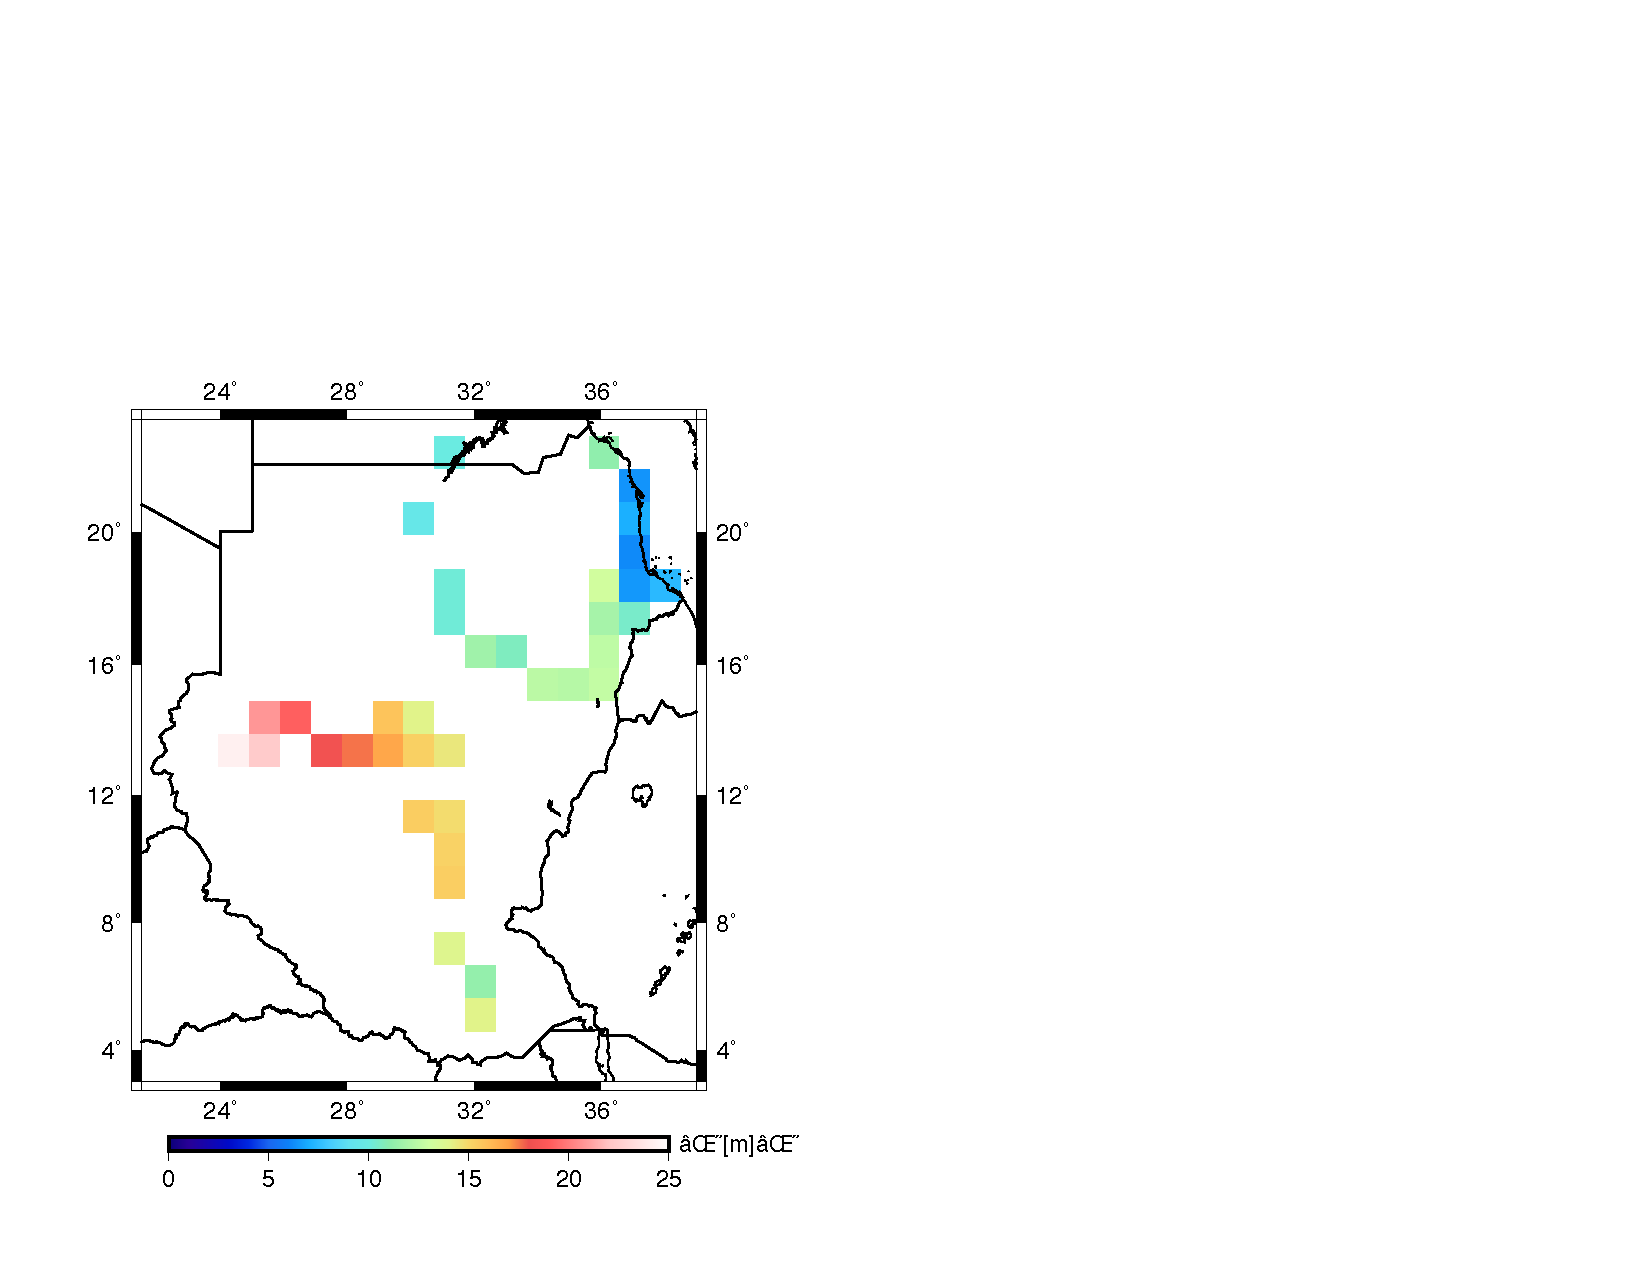
\includegraphics{Figures/points_astro_dist.pdf}
      	\centering
      \end{figure}
      
    \begin{figure}[t]
          	\caption{New geoid model for Khartoum \cite{ahmed_msc}}
          	\label{figure:point_gps_dist}
          	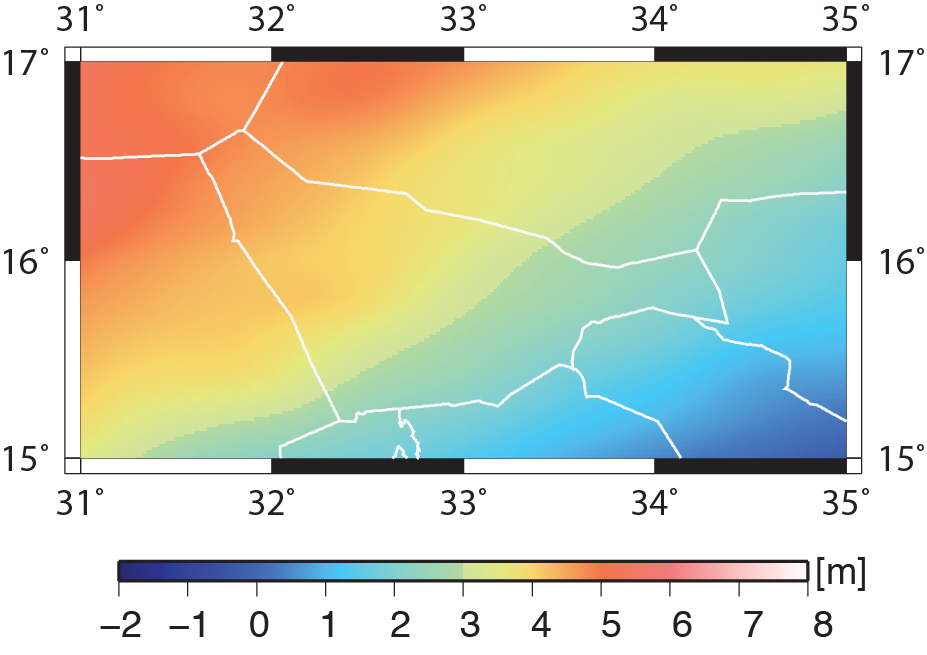
\includegraphics{Figures/krt.png}
          	\centering
    \end{figure}
    
        \begin{figure}[t]
        	\caption{New Geoid for Sudan based on EGM2008}
        	\label{figure:datum_egm2008}
        	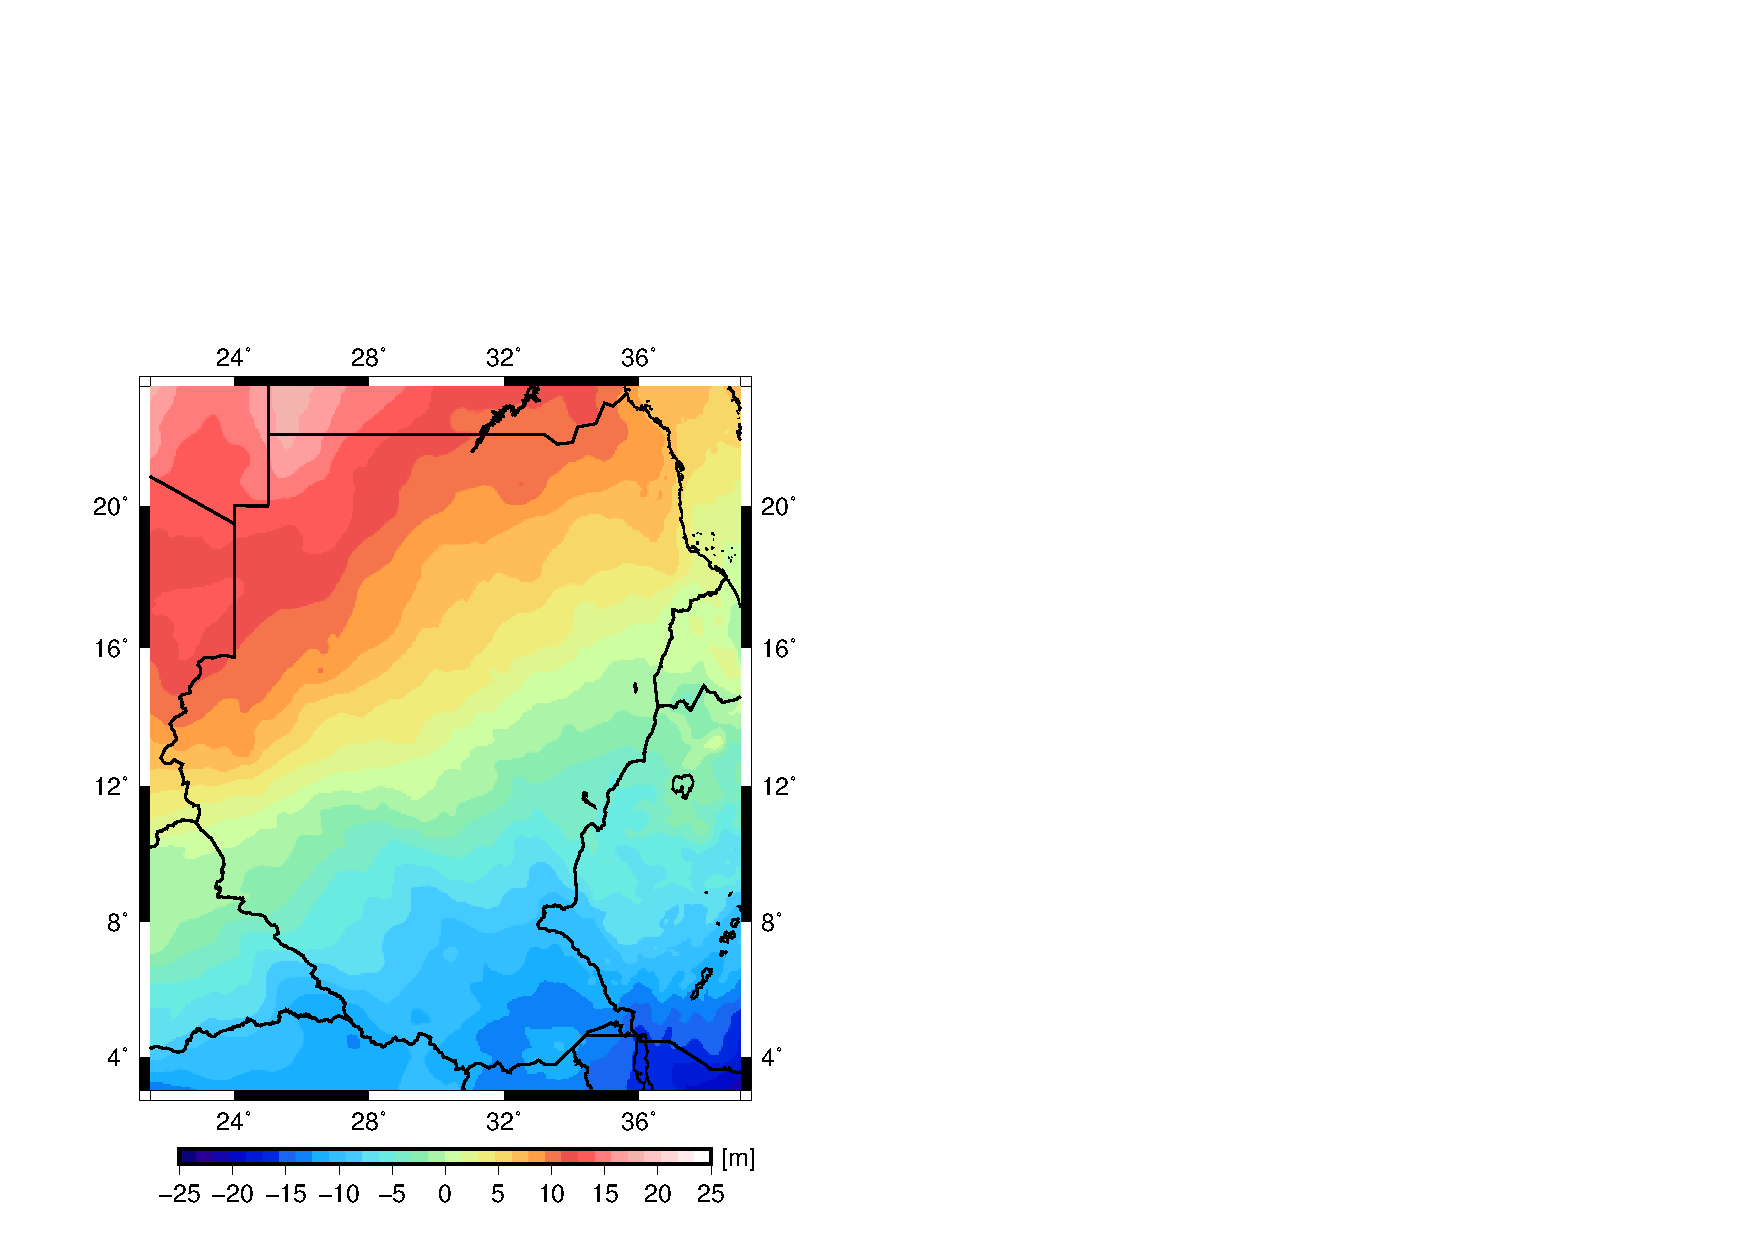
\includegraphics{Figures/cropped_egm2008.pdf}
        	\centering
        \end{figure}
        
        \begin{figure}[t]
              	\caption{New Geoid for Sudan based on EIGEN-6C4}
              	\label{figure:datum_eigen6c4}
              	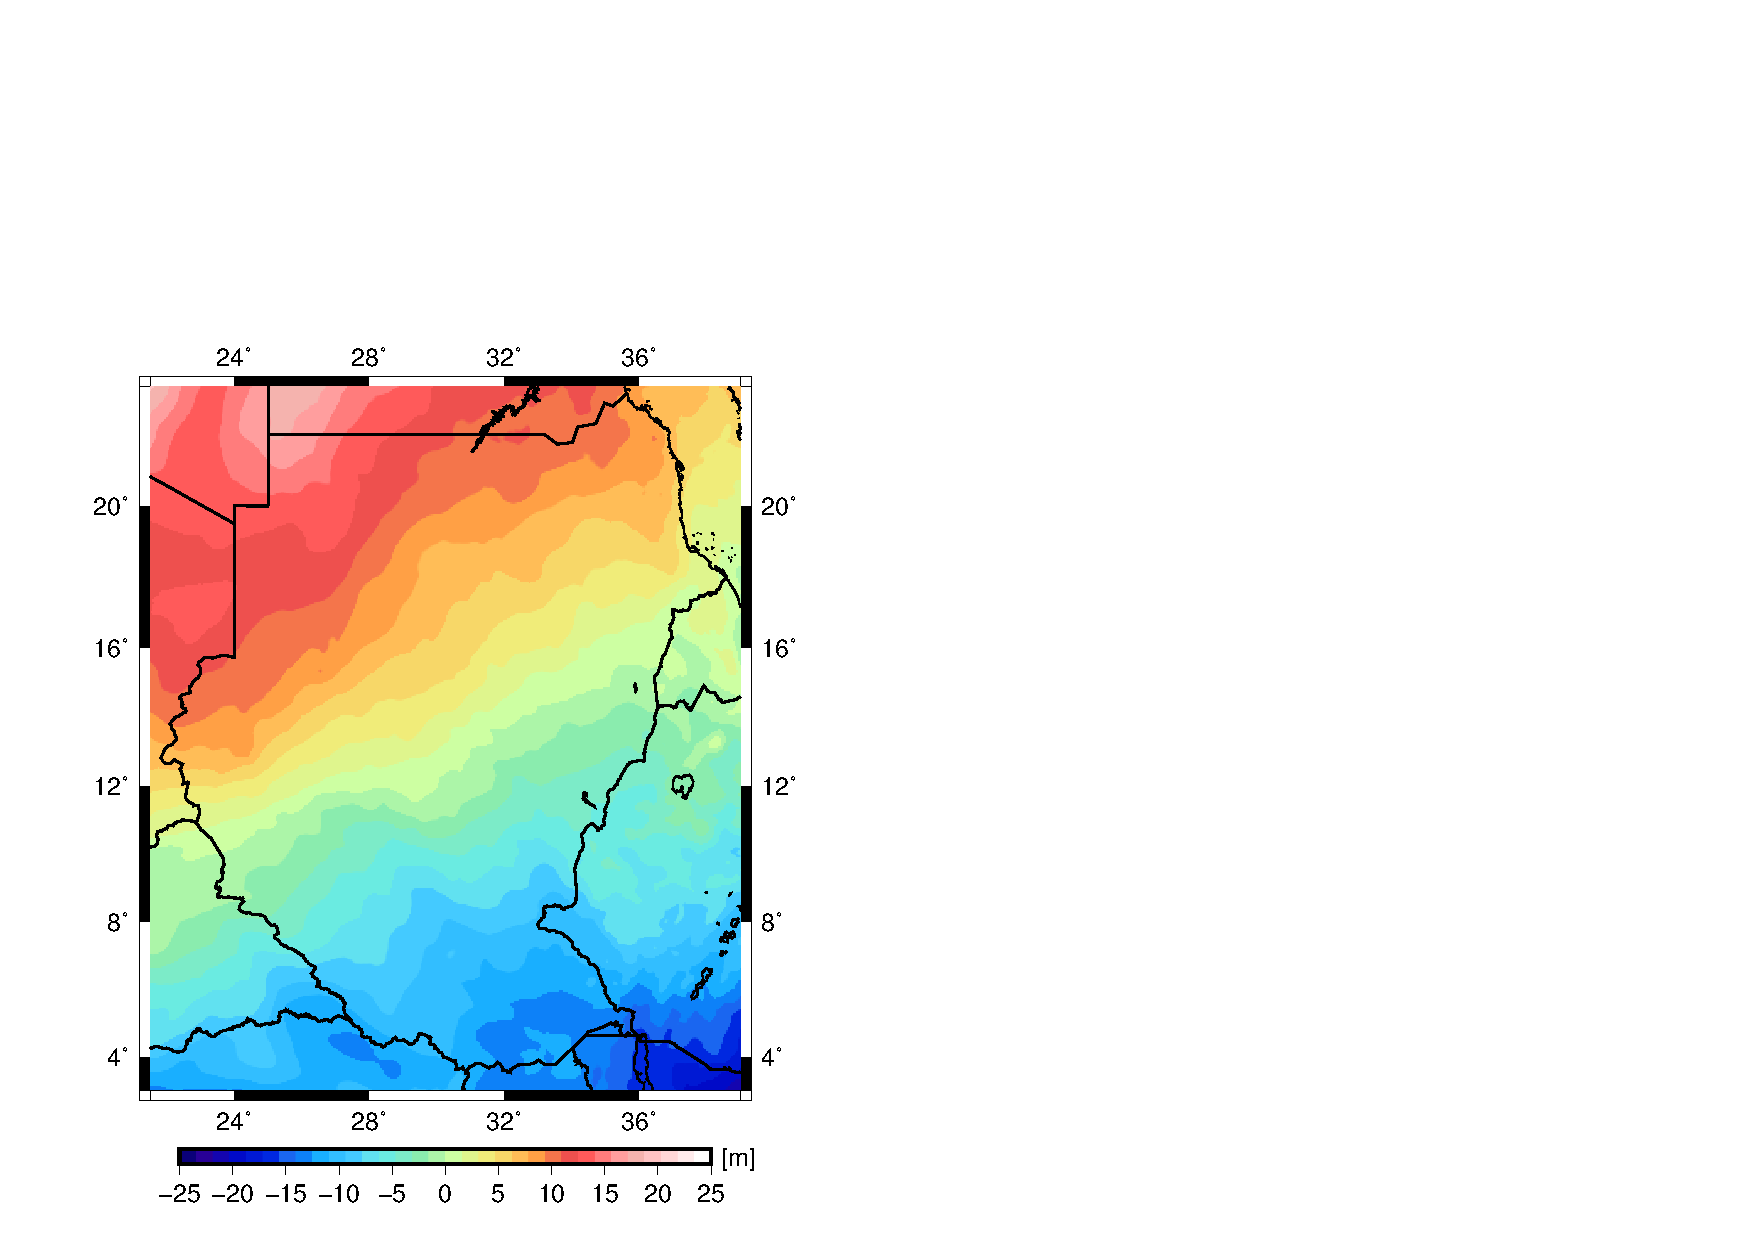
\includegraphics{Figures/cropped_eigen6c4.pdf}
              	\centering
        \end{figure}
        
            \begin{figure}[t]
                  	\caption{New Geoid for Sudan based on GECO}
                  	\label{figure:datum_geco}
                  	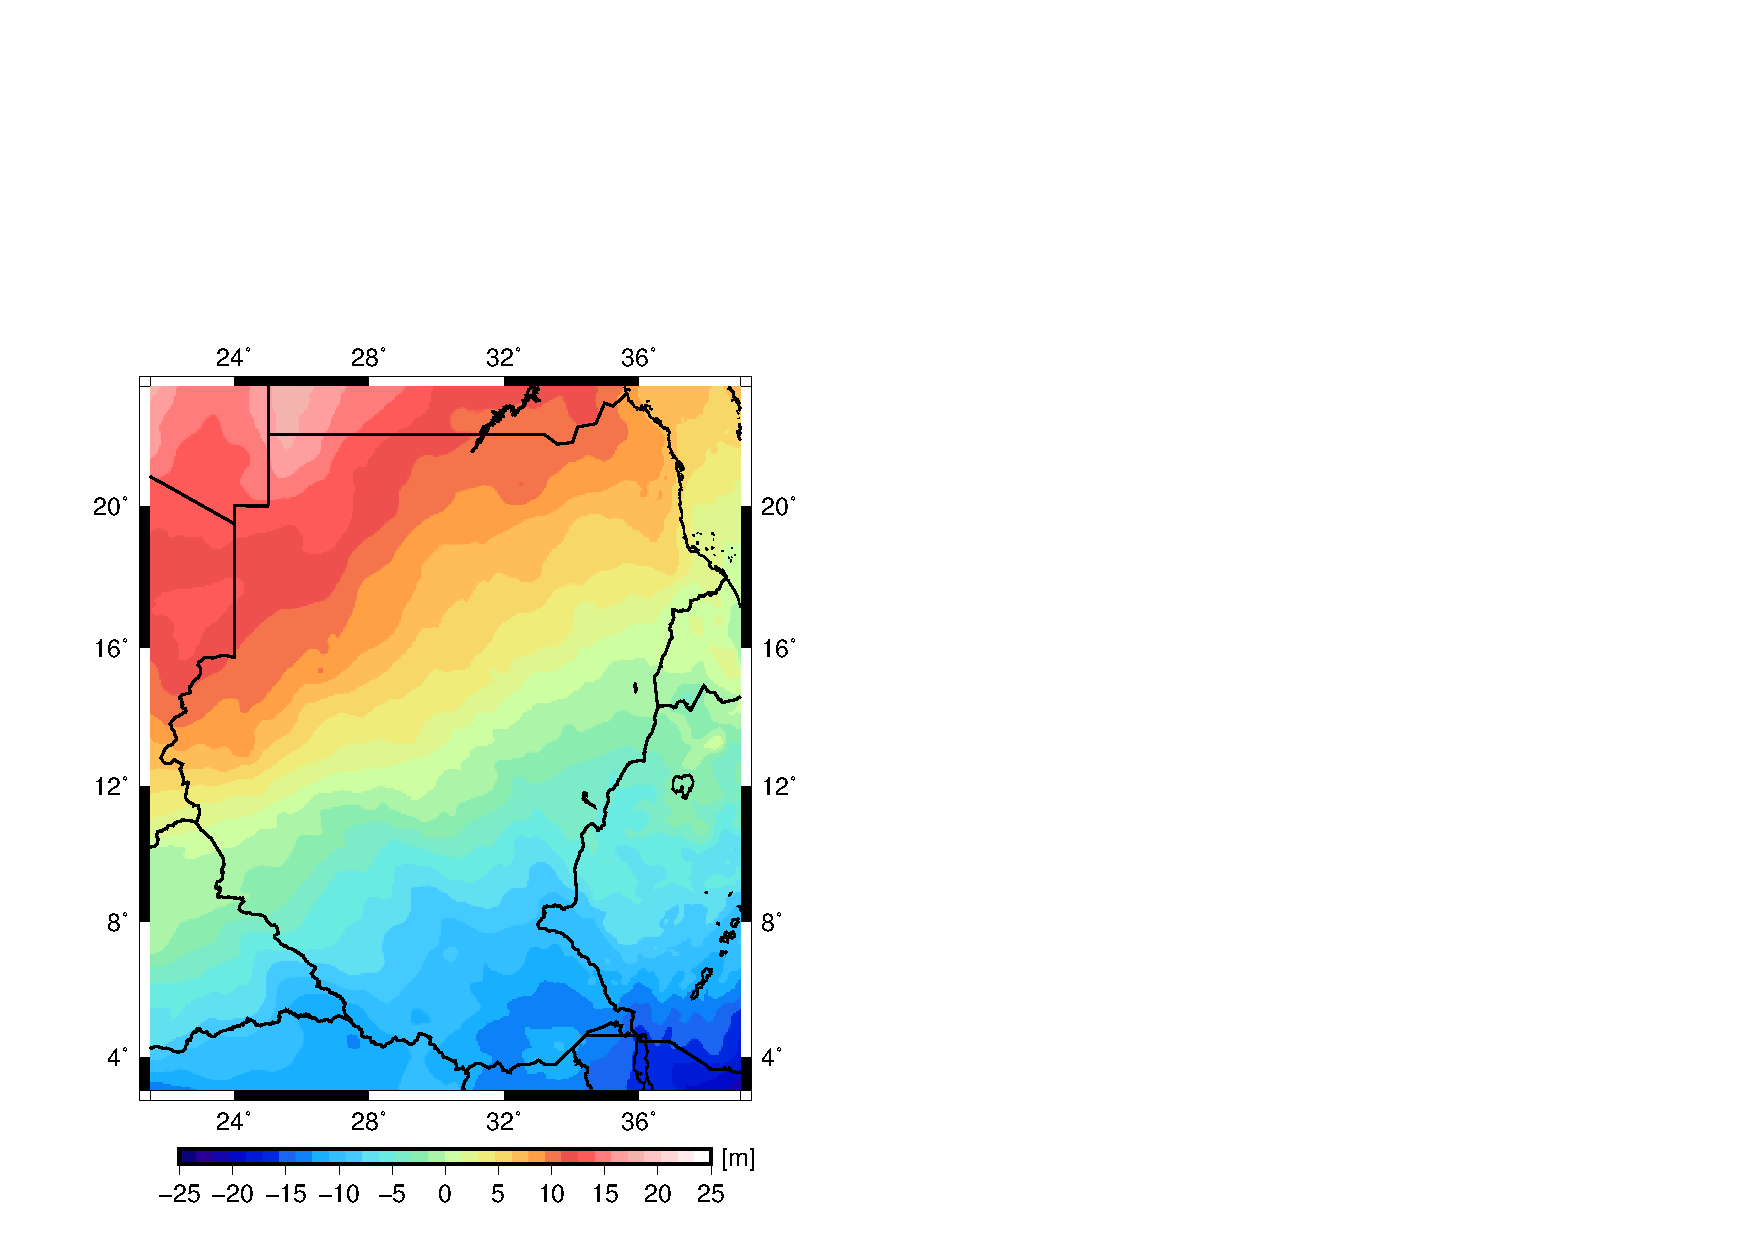
\includegraphics{Figures/cropped_geco.pdf}
                  	\centering
            \end{figure}
            
On Fig. \ref{figure:datum_itugrace16}, it is clear that ITU\_GRACE16 has a different behavior than other models. They \cite{itugrace16} reported that ITU\_GRACE16 is not regularized or constrained in any way, the errors increase with degree.Hence, they don't recommend to use it in any work without smoothing. 
                    \begin{figure}[t]
                       	\caption{New Geoid for Sudan based on ITU\_GRACE16}
                       	\label{figure:datum_itugrace16}
                       	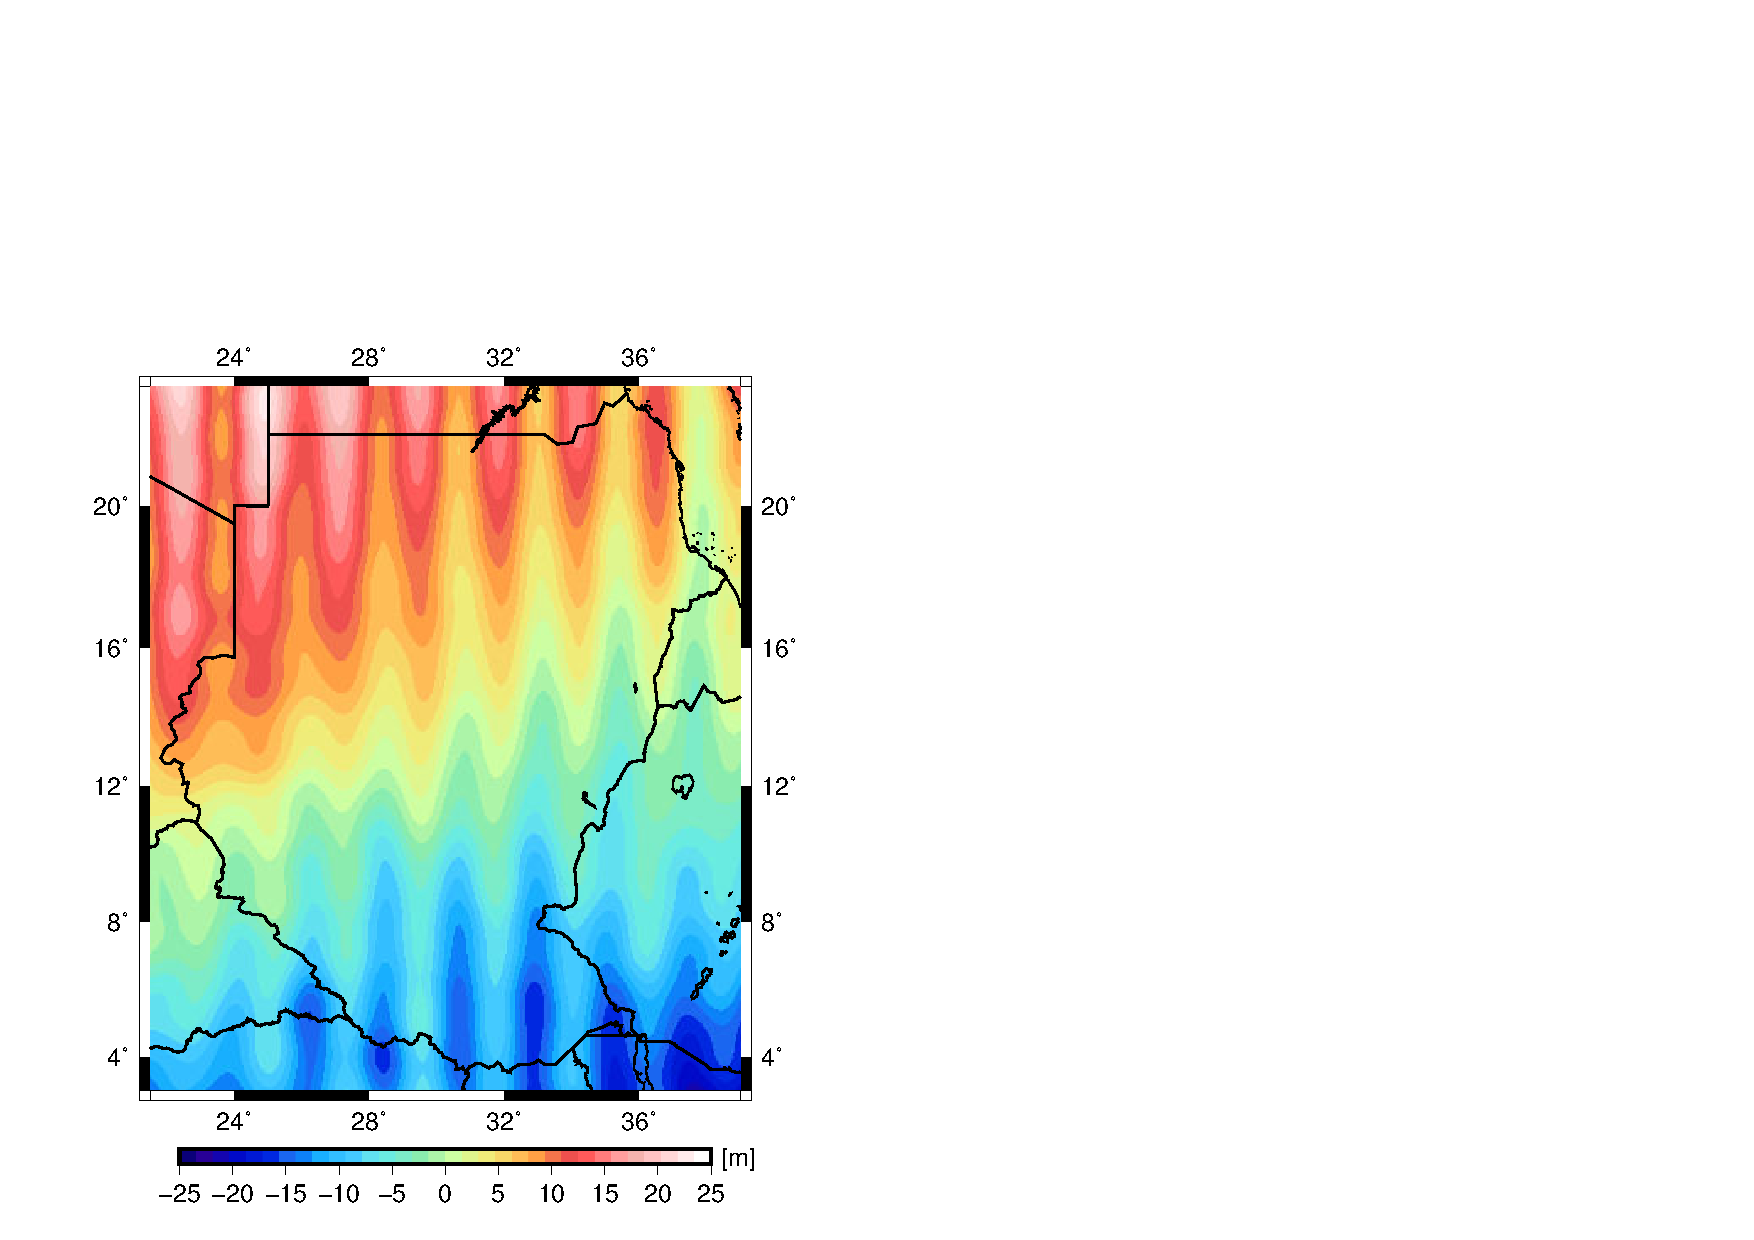
\includegraphics{Figures/cropped_itu_grace16.pdf}
                       	\centering
                    \end{figure}